\documentclass{standalone}
\usepackage{pgfplots}
\usepackage[charter]{mathdesign}
\begin{document}
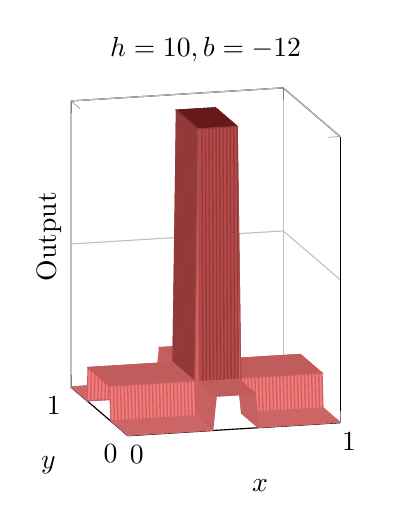
\begin{tikzpicture}[declare function = {sigma(\x)=1/(1+exp(-\x));step(\x,\s,\t) = 0.5*sign(\x-\s)-0.5*sign(\x-\t);}]
	\begin{axis}[colormap={justred}{rgb255=(255,127,127);rgb255=(127,31,31)},grid=major,width=5cm,height=6cm,view={-15}{10},xlabel={$x$},ylabel={$y$},zlabel={Output},title={$h=10,b=-12$},zmin=0,zmax=1,xtick={0,1},ytick={0,1},zmajorticks=false]
		\addplot3[surf,domain=0:1, samples=61, shader=faceted]{sigma(10*(step(x,0.4,0.6)+step(y,0.3,0.7))-12)};
	\end{axis}
\end{tikzpicture}
\end{document}
		